\FloatBarrier
\chapter{Basisbegrippen}
\label{sec:Basisbegrippen}

	\FloatBarrier
	\section{Inleiding}
	\label{sec:Basisbegrippen Inleiding}

Een bepaalde hoeveelheid flu\"idum zal steeds bestaan uit een zeer groot aantal moleculen. De hoeveelheid moleculen binnen \unit{1}{m^3} water bij atmosfeer druk en 20\textcelsius\ is ongeveer \unit{10\times10^{30}}{}. Een theorie die het gedrag van al deze moleculen zou voorspellen, bijvoorbeeld op basis van deeltjesmechanica, zou zeer complex zijn en weinig praktish nut hebben aangezien de rekencapaciteit van huidige supercomputers verre van voldoende zou zijn om zulke systemen op te lossen.
\npar
We moeten dus methodes bedenken om het globale gedrag van zulke systemen te beschrijven.
\npar
In dit hoofdstuk worden enkele principes die het mogelijk maken om flu\"ida te bestuderen.
	
	\FloatBarrier
	\section{Beschrijving van een continu\"um}
	\label{sec:Beschrijving van een continuum}	
We zullen binnen de flu\"idomechanica een flu\"idum niet bestuderen als een verzameling van moleculen maar als een continu\"um. Deze benadering is analoog aan degene gebruikt binnen de vaste stof mechanica.
We smeren als het ware de moleculen binnen het flu\"idum uit over de volledige ruimte die het flu\"idum inneemt (en niet enkel de ruimte die bezet wordt door de afzonderlijke moleculen). Dit brengt met zich mee dat alle afgeleide principes enkel geldig zijn indien we een volume beschouwen waarin voldoende moleculen aanwezig zijn zodat de gemiddelde eigenschappen van de aanwezige moleculen representatief is.
\npar
Beschouw als voorbeeld een bepaald volume uit een flu\"idum. Aangezien de moleculen in een flu\"idum een grote bewegingsvrijheid hebben zullen er steeds moleculen het volume in en uit bewegen. Wanneer het beschouwde volume echter groot genoeg is zullen er steeds ongeveer evenveel moleculen binnen het beschouwde volume zijn (de beweging van de moleculen is willekeurig dus zullen er evenveel moleculen instromen als uitstromen). De massa van het water binnen het volume is dus ook constant. Wanneer het volume echter zo klein gekozen wordt dat er slechts enkele moleculen zich binnen het volume bevinden heeft de verplaatsing van \'e\'en enkele molecule een veel groter effect op de variatie van massa binnen het volume en kan de continu\"um aanname niet meer gerechtvaardigd worden.
\npar
%Beschouwen we nu een ander voldoende groot volume binnen hetzelfde flu\"idum. Binnen dit volume zullen zich een andere hoeveelheid moleculen bevinden. Het volume zal dus ook een andere massa hebben. Zelfs indien de verdeling van de moleculen binnen het flu\"idum overal gelijk is, is de massa van het beschouwde volume afhankelijk van de grootte van het volume. We kunnen de eigenschap massa dus niet gebruiken om variaties binnen het flu\"idum te beschrijven. Een oplossing voor dit probleem is echter zeer voor de hand liggend. Indien we de massa van het flu\"idum binnen een beschouwd volume delen door het volume bekomen we een eigenschap die onafhankelijk is van het beschouwde volume. Deze eigenschap wordt \emph{dichtheid} genoemd:

Een belangrijke eigenschap voor het beschrijven van een continu\"um is de \emph{massadichtheid} of \emph{dichtheid}. Deze wordt gedefinieerd als de massa binnen een bepaald volume gedeeld door het ingenomen volume wanneer dit volume infenitesimaal klein wordt. 
\begin{equation}
	\rho = \lim_{\delta V \to 0} \frac{\delta m}{\delta V}
	\label{eqn:dichtheid}
\end{equation}
Onder de continu\"um aannames zal de dichtheid onafhankelijk zijn van de grootte van het infenitesimaal volume. En heeft de bovenstaande limiet een constante waarde. De SI eenheid van dichtheid is \unit{}{kg/m^3}.
\npar
In de mechanica zijn we steeds geinteresseerd in de beweging en vervorming van systemen onder invloed van krachten. In de continu\"um veronderstelling kunnen we deze krachten onderverdelen in \emph{volumekrachten} en \emph{oppervlaktekrachten}. De meest voor de hand liggende volume kracht is de zwaartekracht. Deze zal overal in het continu\"um aangrijpen en is gelijk aan het product van de massadichtheid en de valversnelling. De totale kracht die een volume kracht uitoefend op een systeem kunnen we berekenen door de volume integraal van de volumekracht over het volledige volume te nemen (vandaar de naam). Zo wordt de totale zwaartekracht uitgeoefend op een systeem:
\begin{equation}
	\vt{F_{g,totaal}} = \int_V \rho \vt{g} \diff V = m \vt{g}
	\label{eqn:volumekracht}
\end{equation}
In tegenstelling tot volume krachten zullen oppervlaktekrachten enkel aan de rand van een volume inwerken. Deze kunnen beschreven worden door de spanning op een oppervlak. De spanning noteren we met het symbool $\sigma$ of $\tau$ en heeft een eenheid  \unit{}{N/m^2}. De totale kracht die een spanning op een oppervlak uitoefent wordt berekend als: 
\begin{equation}
	\vt{F_{\sigma,totaal}} = \int_A \vt{\sigma} \diff A
	\label{eqn:oppervlaktekracht}
\end{equation}
De spanning op een oppervlak kan steeds beschreven worden door een component loodrecht op het oppervlak, de \emph{normaalspanning} $\sigma$ en een component tangentieel aan het oppervlak,de \emph{schuifspanning} $\tau$ (Figuur \ref{fig:spanning}).
\begin{figure}[htb]
	\centering
	\includesvg{fig/basisbegrippen/Spanning}
	\caption{Spanning aan het oppervlak van een continu\"um}
	\label{fig:spanning}
\end{figure}

	\FloatBarrier
	\section{Beschrijving van een flu\"idum}
	\label{sec:Beschrijving van een fluidum}
Beschouw twee starre evenwijdige platen op een bepaalde afstand van elkaar met een bepaalde vloeistof ertussen (Figuur \ref{fig:Evenwijdige platen}). De onderste plaat staat vast opgesteld, terwijl de bovenste plaat kan bewegen zoals aangegeven op de figuur. Indien we een kracht $F$ uitoefenen op de bovenste plaat zal deze is dezelfde richting gaan bewegen. De uiteindelijke snelheid waarmee de plaat beweegt zal afhankelijk zijn van de uitgeoefende kracht.
\begin{figure}[htb]
	\centering
	\includesvg{fig/basisbegrippen/Viscositeit_platen}
	\caption{Evenwijdige platen met een vloeistof }
	\label{fig:Evenwijdige platen}
\end{figure}
Wanneer we de kracht uitoefenen zoals aangegeven introduceren we een spanning in de vloeistof met grootte $\tau$:
\begin{equation}
	\tau = \frac{F}{A}
\end{equation}
Met $A$ de oppervlakte van de vloeistof in contact met \'e\'en van de platen. Aangezien deze ervoor zal zorgen dat de twee platen tenopzichte van elkaar gaan schuiven wordt hierdoor de naamgeving schuifspanning ook duidelijk. Indien we een schuifspanning op een vaste stof zouden uitoefenen via de twee platen, dan zouden deze over een bepaalde afstand $\delta$ verschuiven en dan tot stilstand komen. Bij een vloeistof zal de beweging echter niet stoppen. Hieruit volgt ook de definitie van een flu\"idum:

\begin{quotation}
	Een flu\"idum is een stof die onder invloed van een eindige kracht een oneindige vervorming aanneemt.
\end{quotation}

In de vaste stof mechanica wordt de vervorming tot de spanning gerelateerd door de elasticiteitsmodulus of de glijdingsmodulus. Aangezien er in de flu\"idomechanica sprake is van oneindige vervormingen is een zelfde aanpak niet mogelijk. Een andere aanpak is de vervormingssnelheid te relateren tot de schuifspanning. Als in het beschouwde voorbeeld de bovenste plaat een snelheid $v_0$ heeft dan zal een deel van de vloeistof dat op tijdstip $t$ een rechthoekige vorm had er op een tijdstip $t+\Delta t$ eruitzien als een parallelogram (Figuur \ref{fig:Vervormingssnelheid}). We kunnen we de vervormingssnelheid uitdrukken als de verandering van de hoek $\alpha$.
\begin{figure}[htb]
	\centering
	\includesvg{fig/basisbegrippen/Viscositeit_vervormingssnelheid}
	\caption{Vervormingssnelheid}
	\label{fig:Vervormingssnelheid}
\end{figure}
Uit experimenten blijkt dat in de buurt van een wand elk flu\"idum de snelheid van de wand aanneemt. De snelheid van de vloeistof aan de bovenwand is dus ook $v_0$. De vervormingssnelheid wordt dan:
\begin{equation}
	\text{vervormingssnelheid} = \lim_{\Delta t \to 0} \frac{\alpha}{\Delta t} \simeq \lim_{\Delta t \to 0} \frac{\delta}{h \Delta t} = \frac{v_0}{h}
\end{equation}
Wanneer het snelheidsprofiel niet lineair is kunnen we deze uitdrukking veralgemenen tot:
\begin{equation}
	\text{vervormingssnelheid} = \frac{\diff v}{\diff y}
\end{equation}
De eenvoudigste relatie tussen vervormingssnelheid en schuifspanning is een lineaire relatie. Het verband wordt dan:
\begin{equation}
	\tau = \mu \frac{\diff v}{\diff y}
	\label{eqn:schuifspanning newtoniaans}
\end{equation}
De evenredigheidsfactor $\mu$ wordt de \emph{dynamische viscositeit} of gewoon \emph{viscositeit} genoemd. Vloeistoffen die aan (\ref{eqn:schuifspanning newtoniaans}) voldoen worden \emph{Newtoniaanse} vloeistoffen genoemd. Vele praktische en ingenieursvloeistoffen als water, lucht, smeerolie,... voldoen zeer goed aan deze relatie.
\npar
De viscositeit van een vloeistof is vaak sterk afhankelijk van de temperatuur. Wanneer we de Figuur \ref{fig:dynamische viscositeit temperatuur} bestuderen valt op dat bij vloeistoffen de viscositeit daalt bij stijgende temperatuur, terwijl bij gassen de viscositeit stijgt bij stijgende temperatuur. Dit kunnen we verklaren door op te merken dat bij vloeistoffen de verschillende moleculen dicht bij elkaar gelegen zijn. De viscositeit wordt dus hoofdzakelijk veroorzaakt door intermoleculaire krachten of cohesie. Bij hogere temperaturen nemen deze cohesiekrachten en dus ook de viscositeit af. Bij gassen is de afstand tussen de moleculen groter en de moleculen bezitten elk een willekeurige snelheid. De viscositeit wordt dus veroorzaakt door impulsoverdracht door de moleculen. Aangezien bij stijgende temperatuur de moleculaire activiteit toeneemt zal ook de viscositeit toenemen.
\begin{figure}[htb]
	\centering
	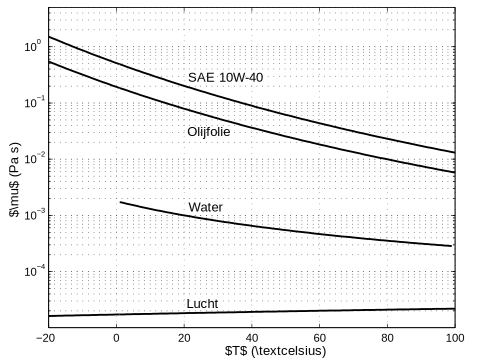
\includegraphics{fig/basisbegrippen/Dynamische_viscositeit_temperatuur.pdf}
	\caption{Viscositeit van verschillende flu\"ida met temperatuur}
	\label{fig:dynamische viscositeit temperatuur}
\end{figure}

	\FloatBarrier
	\section{Beschrijving van een stroming}
	\label{sec:Beschrijving van een stroming}
Wanneer een vloeistof stroomt wil dit zeggen dat er vloeistofdeeltjes zich verplaatsen van \'e\'en plaats naar een andere. Deze beweging van deeltjes kunnen we beschrijven door de positie $\vt{r}$ van elk deeltje te volgen in de tijd. Indien we de positie van een deeltje op elk tijdstip kennen kunnen we ook de snelheid $\vt{v}$ van het deeltje bepalen en kunnen we de stroming karakteriseren. We kunnen dus elk deeltje een label $j$ geven en de snelheid en positie van elk deeltje beschrijven als:
\begin{eqnarray}
	\vt{r} = \vt{r}_i(t) \\
	\vt{v} = \vt{v}_i(t)
\end{eqnarray}
Deze benadering wordt de Langrange benadering genoemd en is bekend van in de deeltjesmechanica. Voor het behandelen van een continu\"um is deze benadering echter niet erg praktisch. De hoeveelheid deeltjes die gevolgd zou moeten worden zou snel hoog oplopen.
\npar
Een andere benadering wordt de Euler benadering genoemd. Hier wordt de snelheid van de stroming beschreven als een vectorveld. Op elk tijdstip wordt op elke positie de snelheid bepaald onafhankelijk van welk deeltje er zich op dat tijdstip bevindt. Voor een tweedimensionale stroming wordt dit:
\begin{eqnarray}
	\vt{v} = \vt{v}(t,x,y)
\end{eqnarray}
Vaak zal het snelheidsveld onafhankelijk zijn van de tijd. Het snelheidsveld ziet er met andere woorden steeds hetzelfde uit. voor een tweedimensionele stroming wordt dit: 
\begin{eqnarray}
	\vt{v} = \vt{v}(x,y)
\end{eqnarray}
We noemen dit een stationaire stroming. Veel stromingen in de ingenieurstoepassingen kunnen als stationair beschouwd worden. De stroming van water door een leiding bijvoorbeeld zal op een inloop en uitloop fenomeen na tijdsonafhankelijk zijn. Ook de stroming door systemen als turbines en compressoren, met inwendig bewegende onderdelen, kunnen als stationair beschouw worden aangezien aan de inlaat en uitlaat de stroming weinig invloed zal ondervinden van het voorbijkomen van roterende onderdelen. Zolang we enkel in de ingaande en uitgaande stroming geinteresseerd zijn is dit geldig. Wanneer we de details van de stroming in een turbine stator en rotor willen bestuderen zullen we deze als niet stationair moeten beschouwen.
\npar
Ook systemen die op het eerste zicht geen stationaire stroming ondervinden kunnen vaak door een slimme transformatie als stationair beschouwd worden. Nemen we als voorbeeld een vliegtuig. Aangezien het vliegtuig zich door de stilstaande lucht verplaatst zal op een gegeven moment de lucht plaats moeten maken voor het vliegtuig en voldoende tijd later terug in rust zijn. De stroming is dus duidelijk niet stationair. Indien we echter de stroming relatief ten opzichte van het vliegtuig bekijken dan zal het snelheidsveld rond het vliegtuig wel stationair zijn (Figuur \ref{fig:stationaire stroming vliegtuig}). 
\begin{figure}[htb]
	\centering
	\includesvg{fig/basisbegrippen/Stationaire_stroming_vliegtuig}
	\caption{Door een goede keuze van assenstelsel kan een stroming als stationair behandeld worden}
	\label{fig:stationaire stroming vliegtuig}
\end{figure}
\npar
Indien ze gekend zijn kunnen de snelheidsvectoren op elk moment grafisch weergegeven worden. Indien we een set lijnen tekenen die op elk punt raken aan de snelheidsvectoren kunnen we ook op deze manier de stroming grafish weergeven. Deze lijnen worden \emph{stroomlijnen} genoemd (E: Streamlines). Als voorbeeld is in Figuur \ref{fig:snelheidsveld} een snelheidsveld gegeven voor een niet viskeuze stroming in een rechte hoek. De snelheidsvectoren worden als pijlen weergegeven op enkele discrete posities. De stroomlijnen zijn weergegeven als streeplijnen.
\begin{figure}[htb]
	\centering
	\includesvg{fig/basisbegrippen/Snelheidsveld}
	\caption{Weergave van het snelheidsveld van een niet-viskeuze stroming in een rechte hoek}
	\label{fig:snelheidsveld}
\end{figure}
Indien we een experimentele stroming willen visualiseren is het opmeten van de snelheidsveld niet eenvoudig. Een eenvoudige manier om een stroming te visualiseren is op bepaalde posities continu kleurstof te injecteren in de stroming. De lijnen die door de kleurstof gevormd worden kunnen weergegeven worden en worden \emph{stroombanen} genoemd (E: Streaklines).
Een andere manier is om op een bepaald tijdstip op bepaalde posities een kleurstof te injecteren in de stroming en het pad van de kleurstof te volgen. We volgen dan als het ware enkele vloeistofdeeltjes als in de Lagrange benadering. De gevormde lijnen worden \emph{padlijnen} genoemd (E: Pathlines).
Bij stationaire stromingen vallen de stroomlijnen, stroombanen en padlijnen samen.

	\FloatBarrier
	\section{(Niet-) samendrukbare stroming}
In deze cursus zullen we enkel stromingen behandelen die als niet samendrukbaar beschouwd kunnen worden.